\section{Kategorien von Vorgehensmodellen}
\label{sec:Kap-2.2}

Konkrete Vorgehensmodelle unterscheiden sich mindestens darin, in welcher Granularität sie die durchzuführenden Tätigkeiten in einem Software\-entwicklungs\-projekt vorgeben. Doch deutlich stärkere Unterschiede zwischen Vorgehensmodellen finden sich, wenn diese unterschiedlichen \textit{Paradigmen} folgen.
\marginline{Paradigma}
Ein Paradigma ist eine grundsätzliche Denkweise/Lehrmeinung, man findet als Synonyme auch die Begriffe Weltanschauung oder Weltbild. Möglicherweise ist Ihnen der Begriff des Paradigmas in der Informatik aus dem Bereich der Programmierung bekannt. Programmier\-sprachen folgen einem Programmierparadigma -- wie zum Beispiel dem objekt-
\linebreak %%% für Druck
orientierten Paradigma --, wenn sie bestimmte im Paradigma festgelegte \mbox{Prinzipien} einhalten.

\begin{figure}[h!]
	\centering
	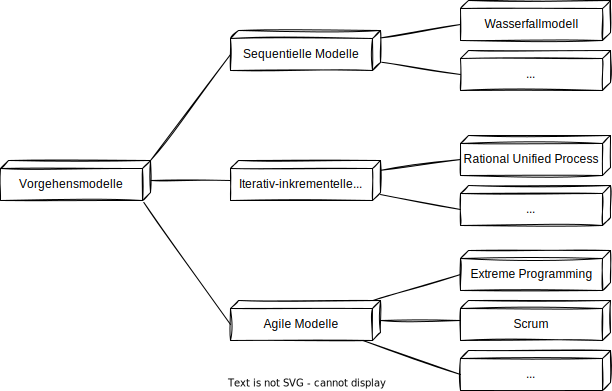
\includegraphics[scale=0.9]{Bilder/Kapitel-2/vorgehensmodelle.pdf}
	\caption{Kategorien von Vorgehensmodellen}
	\label{fig:vorgehensmodelle_komplett}
\end{figure}

Die ersten im Softwareengineering eingesetzten Vorgehensmodelle folgten einem Paradigma, das man als \textit{plangesteuert} bezeichnet. Diesem plangesteuerten Paradigma liegt die Einschätzung zugrunde, dass Softwareentwicklungsprojekte nur dann erfolgreich abgeschlossen werden können, wenn die durchzuführenden (Teil)Prozesse des Softwareengineering und ihr kausal-zeitlicher Ablauf im Vorfeld des Projekts systematisch geplant werden und spätere (Teil)Prozesse immer erst bei Vorliegen von vollständigen, qualitätsgesicherten und dokumentierten Ergebnissen vorhergehender Prozesse starten. Vorgehensmodelle, die dem plangesteuertem Paradigma folgen, gehören zur Kategorie der sogenannten \textit{sequentiellen Modelle} 
\marginline{sequentielle Modelle} 
oder Phasenmodelle. Der bekannteste Repräsentant sequentieller Modelle ist das Wasserfallmodell.

Im Unterschied zum plangesteuerten Paradigma wird im sogenannten agilen Paradigma, das seit Ende der 1990er Jahre verstärkt propagiert wird, die Einschätzung vertreten, dass ein Softwareentwicklungsprojekt nur dann erfolgreich abgeschlossen werden kann, wenn im Projektverlauf Änderungen zugelassen werden können, im Besonderen Änderungen der Anforderungen, und schon ab frühen Zeitpunkten im Projektverlauf lauffähiger (aber auch wieder änderbarer) Programmcode erzeugt wird. Vorgehensmodelle, die dem agilen Paradigma folgen, nennt man 
\marginline{agile Modelle} 
\textit{agile Modelle}. Bekannte Repräsentanten sind Extreme Programming und Scrum.

Sowohl sequentielle als auch agile Modelle werden heute im Softwareengineering eingesetzt. Konkrete Vorgehensmodelle – sowohl diejenigen, die wir in diesem Text vorstellen als auch die vielen anderen, die wir hier nicht thematisieren – passen in der Regel nicht hundertprozentig in genau eine Kategorie, da sie zusätzlich oft auch Kennzeichen anderer Kategorien aufweisen. In der Praxis gilt dies umso mehr, je stärker die Grundform eines Vorgehensmodell individuell an unternehmensspezifische Belange angepasst wird.

Wir werden in den folgenden Abschnitten sowohl allgemeiner die Kennzeichen sequentieller Modelle (Kap.~\ref{sec:Kap-2.2.1}) und agiler Modelle (Kap.~\ref{sec:Kap-2.2.3}) als auch konkrete Vorgehensmodelle als Repräsentanten dieser Kategorien von Vorgehensmodellen vorstellen. Abschnitt~\ref{sec:Kap-2.2.2} thematisiert zwischen der Vorstellung der sequentiellen und der Vorstellung der agilen Modelle eine dritte Kategorie von Vorgehensmodellen, die \textit{inkrementellen und iterativen Modelle}, 
\marginline{inkrementelle und iterative Modelle}
die in den späten 1980er und frühen 1990er Jahren erstmalig vorgestellt wurden und damit auch in ihrer Entstehungszeit zwischen den sequentiellen und den agilen Modellen liegen. Deren zugrundeliegendes Paradigma betont den Stellenwert der fachlichen Aspekte (Strukturen, Geschäftsprozesse etc.) des Einsatzgebiets des zu entwickelnden Softwareprodukts – und kritisiert damit auch die in der Regel sehr technisch orientierte Sichtweise von sequentiellen Vorgehensmodellen. Zum anderen beinhaltet es die Einschätzung, dass für erfolgreich durchzuführende Softwareentwicklungsprojekte lauffähiger Programmcode nicht erst am Ende des Projekts vorliegen darf – hier wurde die Basis für die Programmcode-Fokussierung der späteren agilen Modelle gelegt. 

\minisec{Unterscheidungsmerkmale zwischen Vorgehensmodellen}

Sequentielle, iterativ-inkrementelle (synonym: inkrementell-iterativ) und agile Vorgehensmodelle unterscheiden sich vor allem in folgenden Aspekten, die wir bei der Vorstellung der drei Kategorien in den folgenden Abschnitten jeweils im Detail betrachten werden:

\begin{enumerate}
	\item In welcher Weise werden die einzelnen (Teil)Prozesse zum Softwareentwicklungsprozess zusammengestellt?
	\item Wie wird mit neuen oder veränderten Anforderungen während der Entwicklung umgegangen?
	\item Inwieweit werden Auftraggeber und zukünftige Nutzer des zu erstellenden Softwareprodukts in die Entwicklung einbezogen?
	\item Zu welchen Zeitpunkten liegen auslieferungsfähige Produkte bzw. Teilprodukte vor?
	\item Welche Formen von Artefakten (\zb Programmcode, Dokumente, Modelle) entstehen im Laufe des Softwareentwicklungsprozesses?
\end{enumerate}
